\documentclass[11pt]{amsart}
\usepackage{graphicx}

\begin{document}

\title{Hackerspaces on the West Coast and in India}
\author{Kevin Vilbig}
\maketitle

I am going to be using an ethnography, participant observation, as the basis for this study. This document is my daily notes from the experience. This is an ethnographic exploration into this phenomenon of shared, communal workspaces for groups that call themselves Hackers. Hence, these places are known as Hackerspaces. This project will include some snapshot demographics (by activity, not incidental characteristics) of attendance at a number of these self-proclaimed hackerspaces. I have found evidence of these spaces all over the world from online registries.

I will be collecting quantitative data on the use of the hackerspaces while I am there. What are people actually doing in these Hackerspaces? This will include attendence broken up by the type of project being worked on, whether the person self-identifies as a hacker etc. I will weave this with qualitative interview-based information about the people's use of and interests relatiing to hackerspaces. I am exploring some other media collection possibilities as well. I mean I’m going to see if I can also get some quality video or audio, or even just photographs. That depends on my funding options and other constraints.

I will be doing this research over the course of the winter term as an Honors Research Project. Lee Shaker is advising me on this project.

I leave on a train, Sunday.

\section{Jan 14th- Day 1 in San Fransisco}

I arrived early this morning in town after a 17 hour train ride. I ate some food and walked around the city, seeking my accomadations. I had it in mind to make my way to Noisebridge at ~5pm after getting settled, showered, and otherwise recovered from the train ride. When I woke up at 11pm. and went back to sleep until about 1am. I realized that was not going to happen today. Dozing on a train ride is not a restful experience, and I obviously needed a real chunk of rest in order to continue. What I did instead, after grabbing a late-night snack,  is do a thorough read-through of the Noisebridge website, and found that at 8pm tonight, there will be a weekly governance meeting.

Also, on the train, I met a PhD student who is married to someone in the Computer Science dept. at  Berkeley. I am going to e-mail her today and see what can be done with that connection.

\section{Jan 15th - Day 2 in San Fransisco}

Tonight took a bit of a different spin from what I expected when I hopped on the 14 bus line down Mission St. I still went to the hackerspace. I still opened up my laptop. There were people there. The difference comes down to the focus of the proceedings. This was not a night of programming and teaching classes, though there was a class of fourteen people (and one dog) learning about hacking together some rudimentary Ruby on Rails code to get a simple clone of twitter up and running. The main event of the evening was not this, however.

Tuesday nights hold the governance meetings for the consensus-run space. During these meetings, the members sit down around a table and discuss the business of the space. Unfortounately, much of that business this evening included banning certain folk from entering the space. One forever, period. He was most definitely mentally ill in some ways, I don't quite know how, but some time prior to today he caused a major disturbance, accusing the people around him of being FBI before calling the police on himself. I don't know the whole of the events. Regardless, he's out for good. The other two have a chance to redeem themselves, but that seems unlikely, as they had a long history of decisively un-excellent behavior.

Yeah.

It was that kind of meeting.

There was a lot else that went on during the meeting. Some of it lighter hearted (Christopher Walken shaped chocolates?), some of it serious business ( possible deal to licence out some of their IP to a movie studio. Very helpful, as they are going through a bit of a budget crunch at the moment.

We also talked about the kid from MIT, Aaron Swartz, who recently killed himself rather than face the prospect of fifty years in prison for downloading JSTOR articles that he had license to, being an MIT student and all. (Though he did write a program that downloaded *every* article JSTOR had in it's archives) I spoke briefly with an associate of his from MIT. I plan to go to his memorial here in SF, tomorrow.

I thought this project was going to be simple. I thought it was going to be about people writing programs or teaching other people how to solder. It's not going to be any of that. There are much deeper things going on. It really seems that there is a global network of communities, and individuals, who are looking to challenge the status quo when it comes to how governments and other institutions treat these issues. Two of those in attendance were classmates with Aaron, otherwise visiting SF.

I don't know how far this is going to go, but it's already opening up a really serious conversation about the reach of institutional power.

\section{Jan 16th - Day 3 in San Fransisco}

Today did not quite go as planned. I expected to be attending Aaron's memorial at the moment, but circumstance intervened and instead I'm doing some laundry and typing this up. I spent a good chunk earlier at the public library working on my thesis, and got a lot accomplished. I went to try to find the place, got turned around, harassed by a persistent panhandler that followed me for a few blocks and then realized that I was somewhat underdressed to attend a memorial service. A sweaty t-shirt, jeans and a torn coat don't quite suffice for a respectful costume. There are worse things than missing an event I only heard about yesterday. I have another couple of days in town.

Tomorrow I plan to head down to the Computer History museum in Mountain View. This has less to do with my ethnographic project and more to do with my thesis, but I think the two are so inextricably intertwined that it's quite impossible to untangle one from the other. I'm also thinking about sneaking my way around Berkeley on Friday, see if I can't uncover anything interesting there. I'll see if there are any obvious Hacker groups that do their thing on campus with some internet research tonight and/or tomorrow.

It's actually somewhat fortunate that I got the night off. I will make it a point to get another chunk of time at Noisebridge on Thursday, there will be an event with talks, it will last an hour. So I might talk a bit about my projects.

\section{Jan 17th - Day 4 in San Francisco}

Today was pretty cool. I went to the Computer Museum in Mountain View. That ate my entire day, and all of my energy, so I am going to skip the lightning talks event tonight and instead go to Noisebridge for a big chunk of time tomorrow to hang out, be cool, and do stuff. Prior to now, I was thinking about making it to Berkeley or Stanford tomorrow, but I think it will be better if I save those for a later trip down here. My motivation for going to the universities are mostly driven by their archives of material regarding the people I am studying for that project. It will probably behoove me to make a proper week long research trip to dip into their respective archives of primary source material. It was about an hour's train ride and about an hour of walking to get to the museum (and then back, and then I spent 4 hours walking around in the museum). Mountain View doesn't have the same caliber of public transport as SF proper.

The highlights of the museum include learning more about their research archives. They have access to some material that I have otherwise not been able to find copies of.  I also was informed that Saturday, which is my last day here in SF, they will have one of the original MIT hackers demonstrating the first computer game ever created, Spacewar. I don't think I can pass that up, and ultimately, it's a place where the first generation of hackers are congregating, around the exact same machine (restored) that they used to hack on in the 60s. I can't really complain about an opportunity like that.

\section{Jan 18th - Day 5 in San Francisco}

Mostly harmless.

\section{Jan 19th - Day 6 in San Francisco}

This is my last day to be in town, but my train doesn't roll out until 9 o'clock this evening. I went to the Computer Museum again to hang out and see a demonstration of the PDP-1, one of the first interactive computers. It's definitely the first interactive computing mechanism that was intended to be used as a full - fledged machine, versus the TX-0 that is more like a big programmable calculator/terminal thing. Anyway, the win that came out of that experience, is that along with the legion of 40 schoolchildren packed into the tiny viewing area in front of the exhibited machine, there was a handful of older hackers, definite. I didn't have to ask any questions because the others were asking the technical bits and bobs. I only wish that we had another hour to pester Peter Samson, but my rental car reservation was already overbudget. It was incredibly worth it, regardless. It's amazing to see how much interactivity they got out of that machine. Also, thinking about the difference between printed paper output to a terminal versus video output, and how ultimately, everything is software at some level...  pixels and all that.

Because I had the extra time to kill this evening before I rolled out. I came down to Noisebridge.8 people on computers, 3-5 sitting around. 5:30pm - 7:00pm Nothing on the schedule

On final thoughts, this space is a safe social space that's run as a pool of sanity in a relatively insane city. I spent a lot of time walking around the streets of SF this week, and the mass of people is overwhelming, especially considering my months of near-hermitude prior to this trip.

\section{Note about Missing Days}

I got back to Portland, broke and tired. The funding I expected to come through for the Seattle leg of my journey seems to have mysteriously vanished into the bureaucratic abyss. That's alright. I spent most of the next two weeks readying myself for the next part and working on my thesis. I have developed a correspondence with Richard Stallman, founder of the Free Software Foundation and GNU Project. I attached my current draft and he actually read it and offered copious notes with citations to his on writings. That is very helping-yes for this whole process.

\section{Feb 5 - Delhi}

India has a number of companies that deal with in-country bookings for travel, tourism, etc. I visited about a half dozen of these offices over the course of the day, from a really, really shady 24 hour place right after I dropped in to the one that finally helped me out with my goals here in India. The first crew whisked me away from the airport, pulled a switcheroo on my car and driver\footnote{I'm not sure why. My original driver, Kumar, cited mechanical troubles, but I doubt that. It seemed very, very prearranged.} Here the fare jumped from the 285 INR I expected (about 6 USD) to 2895 INR. I smelled a grift coming on at this point, and figured then that I would ride it through and see what happened.

Dropped into a foreign city at one in the morning and whisked off past packs of barking wild dogs\footnote{One pack, anyway} into a random office. After an hour of arguing that, no,  I am not going to pay 80 USD a night for hotels, no, I don't care that they are three star, I left. I was prepared to just start walking, but my driver waited and was willing to drive me. Finally, I decided in the ride back to the airport that I wasn't going to pay them the 2895 that they expected. The 24 hour place ended up taking me back to the airport, but dropped me at the departures gate. He attempted to argue for the full fare, but I handed him a 500 INR note and walked away. I figured they deserved some compensation for their time and for the learning experience. I wandered around a bit and tried to get inside so that I could get on the wifi and maybe track down a vendor that was selling power adapters. I had very limited battery time on my computers at that point. Alas, the guard at the door wouldn't let me into the terminal itself, no ticket, but he pointed me to the room for the various ticket counters. This was a waiting room, rows of seats, ticket windows. There was a small cafe window, a vending machine, and an empty chair in the corner. I spent an hour drinking some hot lemon tea\footnote{Which the guy at the window short changed me a 100 INR note for...  fool me once...}. I had been putting off mending my coat pockets that had ripped through. So I whiled away the whiles, waiting for dawn to rear it's head by some light sewing and writing a few notes about the experience I had just had. The sky began to lighten. It was time to go. Compass hanging pendant around my neck, backpack strapped around my torso, I left.

I wandered around outside the airport gate for a few minutes until a man in a military uniform got into an elevator that I had overlooked. I jumped on in and engaged in some elevator chatter. I wandered around the ground level, once getting ushered away from some kind of abandoned terminal area by a few armed guards. There was a spa at the airport, a nice respite for travelers who may not have had time to do so before getting on a plane. I paid the woman at the desk their advertised rate of 500 INR to take a thirty minute shower, did so, and filled my water bottles.  When I was done with my bathing, which felt amazing after two days of sitting in the same clothes, I used one of their public computer terminals to message my friends, who were already in Delhi, and to orient myself on a map. I was going to stay there, and use their internet to get some work done, but the price of 1000 INR for two hours lounge access was too steep. I had snuck my prior quick access. Now it was really time to go.

I now knew it was North West to get into the city, so I headed out on foot. Over the next half-hour a half dozen tuk tuk rickshaw drivers looked at me like I was crazy when I declined their offers for a ride, but ultimately, after being cooped in airplanes and airports for the better part of the past two days, and my previous taxi experience, I didn't want to. I haven't yet taken the time to trace an accurate representation of my route on a map, but I ended up hiking for about two or three hours. North, alongside the Air force base, army base, etc. West as soon as I could, along Chuch Road. Really, I just kept the compass needle vaguely pointed in the right direction. There were regular bus-stops and auto-rickshaw drivers passing. If I needed it, I could get a ride, but I didn't need it, at least until I got to the Dhaula Kuhn metro station soaked to the bone, carrying a couple extra gallons of water soaked into my pack and clothes. I was starting to fatigue after about 5km (as the crow flies, anyway. I estimate 8km from the map I am looking at now) of hiking through monsoon. I needed a break.

Now, the best part of the metro was the RFID implanted plastic token that was my ticket for this train. It was blue, about 2cm across, and I waved it over the sensor after going through a cursory inspection of my person and luggage via X-Ray, and I was in. The next 8km took about 15 minutes, and 60 INR.

Mostly, I started to get a sense of how the markets work in Delhi. I hiked through a number of market districts (I saw about 4). They ranged from a strip-mall looking row of closed stalls to the veritable maze that I'm residing in currently. This place has a thriving market culture, and it seems, somehow, I managed to negotiate my way through it to get what I needed, at the price that I needed it. I found a hotel a half km away from the major train station in Delhi. It is costing me 500 INR a night for a big private room and bathroom, with electricity, and a broken TV. Paradise. It's bigger than the room I stay at on campus.

I spent the bulk of the afternoon at Mr. Wahid's tourist booking office after a young marketeer guided me there from a stall where I could get the various electrical kit that I needed to charge my gear. The marketeer then took me to this office and invited me to Mr. Wahid. I forget his name. He allowed me to spend some time on their computers, plied me with much chai, a delicious lunch, and helped me book my travel and hotel for the next two months. For a nice commission, of course. We also watched some of a streamed (It seemed from a pirate server, but I don't know how copyright law works here) Baliwood movie, Race 2. He has an 8 month old son, and has lived in Delhi for 15 years. One of his buddies bought me some international phone time on his phone, so I was able to call my Mom and talk, I left a couple missed calls and a message, so she called back when she woke up.

Finally, I picked up a cellular modem back at that stall. Because of the documentation requirements for people to get telecom access in India, this took a copy machine, a couple computers, a digital camera/portrait studio and a photo printer. All of these things were within a fifty meters of the tourist booking office. The Indian Gov't doesn't allow anonymous telecommunications. I actually also have to activate my service via Mr. Wahid's line, because a local number has to be attached to the account.

I think though, really, the best part of this day has been the occasional whisper "Hanuman", who is Lord Rama's bearded monkey-king companion. Going into a major festival time in India, I'm being compared to a mythic monkey-king? Okay! I'm going to chomp a pepto and watch a movie on this thing. I grabbed a collection of old TV and movies from 1930ish - 1950ish for times like now.

\section{Feb 6 - Day 2 in Delhi}

Today was an overview of Indian culture through the eyes that the government wants to paint itself as. It was a glorious day with a mix of propaganda, religion, and just a touch of magic. I visited a number of landmarks in Delhi. The Lotus Temple of the [Baihai -misspelled, fix later-], A temple to Lakshmi that was built in the 1930s, Lodi Gardens, Indira Ghandi's shrine, a new Indian Cultural monument called Akshardham that had the most glorious mandalas carved into the ceiling, and the various Indian Parliment buildings. I commissioned a driver/guide to take me around the city, he's also going to take me through the countryside this weekend.

What did this get me as far as my goals on this project?

Outside of the various uniformed types out there. There are distinct cultural groups in India. The Sikhs, Muslims, Hindu's, Baihai (which I didn't know anything about until today, and they're pretty hindu-ey), and then the Westernized folks. It's relatively obvious who is who, because they dress the part.  Sikhs with their turbans and beards, Muslims with their beards and women covering their hair etc. etc. 

The division between the classes is painfully obvious with skinny young men pushing rickshaws uphill loaded with goods while busses and trucks drive by. At the top of the hill, a cunning marketer with a stunning display of oranges, stacked in a stepped pyramid of citrus delishiousness.

I also ran into a strange error message on an ATM tonight, which gives me a look into the possible criminal computer element in the city. The ATM was apparently a computer running an old version of WindowsXP, the message said something like C:/Windows/system32/virus/VirusDelete.vbs not found. I don't really know what that means, but it was interesting. Once I get internet I'll do some research, and change my passwords. I still haven't made it to the hackerspace. I'm going to convince my driver to take me there tomorrow and I can case the joint, check it out, swing on in and start with the magic. 

The most amusing note for the day, being the only red-bearded man in the whole city (probably), I feel like a celebrity might feel. Damn, do the people stare. I actually had a young couple ask to take a series of photographs with me. At first I thought that they wanted me to take photographs of them, but no, they got somebody else to take a photograph of the three of us. I don't know why.

Note: The thing that makes this exploration different than many others. I have not taken any university courses on Indian history.  I've picked up bits and pieces on my own, but my preconceptions are, hopefully, minimal. In reality, this is a fresh look at a culture that I know very little about. Sure, I've read pieces of the Bhagavad Gita.  Sure, I've watched a couple Bollywood flicks. But, there isn't a western academic telling me the way things are, at this point.

Ultimately, I don't know what's going on. I probably won't get much more elucidation by the end of all of this, but maybe a little. Everything might change once I get in touch with the hackers-proper. I'll go in the morning to get my internet up and working and start doing some network exploration as well. I am going to play around with this internet stick a bit now, and then watch the rest of that movie and go to sleep.

\section{Feb 7 - Day 3 in Delhi}

God, I don't even want to write this because it's pretty embarrassing, but I guess this is part of the whole game right? Well, here goes.

I'm pretty sure that the tour office that I've been working with over the past couple days is a scam of some kind.  I think the same about the place where I got this Mblaze cellular modem. The two shops seem to be connected by this little gang. I called MTS myself from the phone and they haven't even recieved my paperwork and don't even know what I'm talking about when I ask. The guys at the shops were telling me that it would be ready by 6 or ready by 10 tonight, but I very much doubt that. I also did some sleuthing online, and they don't show up in any of the Indian government's webpages and the site they have listed is really attack-sitey, and they have a bunch of suspicious reviews that come up on Google. So, I'm going to go to the US Embassy and maybe after, the Delhi Police, to talk with some experts about how I should proceed from here. I've given the bastards about 15,000 INR at this point, which is a decent chunk of change, but not totally terrible. I don't really expect it back at this point, but who knows, maybe the best thing to do will turn out to be asking for my money back. Maybe I will just cut my losses and move on. I don't like that these criminals have my picture, passport, and a lot of information about me, but I guess them's the breaks. I am going to change hotels tomorrow also, because the drivers are going to be looking for me here and one of them, frankly, seems like a bit of a thug. He told me all about how he sport wrestles and has enough sign of cauliflaeur ear to prove it. If you don't know what that is, it's a relatively common condition among wrestlers that results from repeated impact damage, even through the padded headgear. I got back home and packed all of my stuff. I was about ready to bolt tonight, but tomorrow is a Free day, and I'm supposed to be going around the city a bit. I've also let them know that I know my way around well enough and though they might expect me to drop by their office tomorrow, I don't think they will expect me to slip out, change hotels, and go to the authorities.

So, I've found some people that grift money out of tourists who go so far as to falsify hits on Google. The Google results would have been convincing if I wasn't so net-savvy, and the average joe wouldn't necessarily think to check the Indian government's websites directly. india.gov.in is a really expansive site. It took me a good half-hour to find the information, but they have a database of every tourist booking company in the country. They also have easy-to-book train tickets online and I don't have to do anything else but take a train and find hotels wherever I go. The problem was, the day that I got involved with these dudes it was raining torrentially and I just wanted to get a damn place and get dry, so I didn't really think much about it. I was still a little bit in shock, jet lagged, and exhausted.

Also, it turns out that AT\&T decided to block my SIM for some unknown reason. I've been getting a weird error on my phone and it won't connect to the network. I asked my Mother to talk to AT\&T about it, as we share a plan, because otherwise I wouldn't have a phone at all.

In almost good news, I got to right near the hackerspace, but wasn't able to find it. I thought I had an address, but I didn't have the right place. They keep the address hidden off of the web and force people to contact them to negotiate entry. I thought that the address that they had on their page was exact, but it points to the Hemkunt Colony, a 2km square residential block in the GK-1 area of New Delhi. Noisebridge, this place is not, but it will definitely be a useful trek. I'm going to get in there as soon as I can, but navigating in a strange city, especially a city like New Delhi, is a challenge. Depending on how my Embassy and Police visits go, I hope to get directions from the people there and start trekking out on the metro and bus lines tomorrow.

Really though, in spite of the mountains of bullshit that I'm going to have to dig through, this was a good day. I got to check out the Library in the national museum that isn't normally open to tourists. It had all of these amazing books about history and archaeology and anthropology and Indian philosophy. I could spend weeks with that collection. I also hit up a couple of great monuments, Mosques from the 12th and 16th centuries.  Ultimately, the up-side of this whole probable-scam-thing is that now, I'm free. This will give me another few days in Delhi to maybe visit the museum library again, and also maybe the Indian Institute of Technology, and maybe actually pull off a look at one of these other hackerspaces as well.

The downside of this whole thing, is I don't really want spurned criminals knowing where I am sleeping at night and I do like this place, maybe because it's tucked into a winding-corridor creepy back-alley kinda place, maybe in spite of that...  maybe because it's 500 INR a night and the TV is broken. But, I'm going to have to move.

I also bought an 8GB micro flash card for 450 INR. The kid in a little stall across from my hotel was trying to get me to sign up for an Indian SIM card with them and I saw a kingston card hanging behind him. You can't really beat the equivalent of 9 USD for something like that.  It was listed at 550 INR, but he dropped the price with a glance. I bet it was stolen, but I don't really care. 

The next couple days are going to be interesting, to say the least.

\section{Feb 8 - Day 4 in Delhi}

So, I still haven't even gotten in contact with the people that I'm ostensibly here to find. This day was a long journey in the morning to the Consulate, and a longer, winding journey back. There are four parts to this exploration.

\subsection{Expert advice from the consulate, reputable wireless dealers} 

The main reason I wanted to get in direct contact with the consulate is to get a reccomendation for a legitimate wireless dealer. I also wanted to see if there was any way to maybe get my money back, but their advice was to just walk away. We have some interesting things to talk about with the journey to the consulate. First, they wouldn't even let me inside the building without an appointment, the security is very tight, pretty much the only thing you can bring inside is yourself, your passport, and maybe some paperwork.  Also, the Embassy is a huge complex with seven or eight gates, all for different purposes, whether diplomatic, citizenry related, etc. The woman I spoke to was aware of my e-mail that I sent yesterday, which is a good thing.

The legitimate dealer that was reccomended to me was in the Malcha Marg Market. It's the Diplomatic enclave here in Delhi. The process was similar to the one with the scammy-shop, but there was paperwork, and I actually have a couple of SIM cards to pop into these devices. They wanted an e-mail address, and my father's name as the security questions when I get everything hooked up. Now, I have two cellular modems of different makes and protocols, and two SIM cards, one for a phone, and one for the data plan. I would have cell and data right now, but I ran into the issue that both my smartphone and the backup cell that I have are still locked by AT\&T. Today, I am going to either buy a new cellphone here in India, or find a way to call AT\&T and get the unlock code for this old Nokia. It will depend on the cost of a phone, or how much hassle it will be to get a phone line to dial out. I have AT\&T's international toll-free number, I think.

It turns out that this project, so far, is less an ethnographic exploration of Indian hackers, but more a chronicle of one lone hacker trying to make my way through this country with not much more than my wits and a prayer.  I hope that there are other good hackers here, and I hope they have some time to hang out.

\subsection{New Delhi Subways}

The subway system here is extensive. It's huge, bigger than any transit system I've seen in America. It's on par with San Francisco's BART, but has more trains, more lines, and during peak volume travel, the most people I have ever seen. It was easy to get a card, 100rs got me a card with 50rs on it, there is a 50rs deposit for the card itself. The trips cost on the order of 10-20rs to get through the subway, and it's all RFID controlled.  One thing about India that's significantly different, probably because of the terror attacks in 2008, the subways have an X-Ray and frisk system like Airports in the US used to have, before we got those contriversial millimeter wave radar systems installed.

\subsection{A little Hack of My Own}

Trying to get back to the Main Bazar from the east side is somewhat difficult, because the train station only allows one local traffic bridge. I was heading the wrong way (which happens a lot) when an old toothless man in a Rickshaw asked if I needed a ride. I took it. He seemed so old that I started worrying that I was killing him, because he probably weighed about 120 pounds. He asked me to hop off and I slipped away, because I thought he was going the wrong direction, he took me back to where I started, pretty much. It turns out that the only reason he asked me to hop off was because he couldn't push me and the rickshaw up the hill. He tracked me down in the crowd, not hard to do, and I gave him a 100rs note for being cool, not for the ride. Then I wandered off in a semi-random direction.

I found some kind of open service entrance to the New Delhi Railway Station. It was an ungated street, wide enough for a couple, maybe three sedans. It was lined with bulldings that were labeled things like "Staff Canteen". There was a steady flow of people, but it was obviously not a major throughfare. After a few hundred meters along this street. I found myself walking by the railways alongside men with wooden and metal carts that could have been made in the 15th century. They were hauling scrap to a big pile of twisted metal girders. I noticed a covered bridge with steps that led to the west, which is where I needed to go. I walked out of the train station through the entry gate and ran into another old man, after winding my way closer to the bazar. He led me to the hotel where I am staying now. It's a little more expensive, but the flat-screen and cable work. So, I got to spend some time last night watching National Delhi, which I think is like PBS here.

\subsection{Walking away}

Here is where I am glad that there are so many people around. I am actually a little worried about this gang of con-men. I think I will be okay, as I was just one kettle on their stove, and honestly, a 15,000 INR score for Mr. Wahir, which is significant in a country where 67\% are getting government assistance with food grains\footnote{Hindistan Times Article, Front Page, Feb 8, 2012} My favorite driver, Raju, said that he only got 5,000 INR salary. That's about \$100 a month. With that, he raised two sons and a daughter. His daughter is a doctor, though.

Anyway, I saw about a half-dozen other tourists during the couple days that I hung out at their office. So, I don't think they are going to be looking too hard. I left some confusing evidence behind, a german newspaper that I picked up in Frankfurt.  I told the man at the other hotel that I was heading to Mumbai next. I'm thinking that I will be changing the focus of this project again, I'm having to wrangle with the dizzying array of phenomena that I run into every time I open my eyes. I think I am going to skip Mumbai completely. I do want to try to go to this Nulcon hacker conference, even though it's not on my proposed plan, because after my experiences here in Delhi, I am certain that it could be an important way to engage with the people that I am looking for, where I can actually, certainly, talk to people about their experiences as being Indian hackers. I'm also going to start doing something very different in my travels. I am going to be jumping onto Couchsurfing.org and getting my profile built and contacting Indian people who are wired and want to hang out with traveler-guests. Getting the experience of what it's like to be an unconnected traveler in Delhi has given me a way to place everything else in context. For that, I thank my con-men brothers. 

\section{Feb 9/10 - Day 5/6 in Delhi}

I'm taking the weekend off from working. This has been a rough week with a lot of time on my feet and I have a lot to process. I am also very behind on my thesis work and need to get some reading done, and throw down a couple pages, but I'm probably not going to get much done because I have a lot to think about.

\section{Feb 12 - Delhi}

I found my friends who are in country. I've also found a nice little case of traveler's diarhea. I know exactly what did it. It's the only questionable thing I've eaten my whole time here. It was some weird pickled fruit of some kind. Don't eat the weird pickle.

\section{Feb 13 - Delhi - Success}

I have finally actually made it to the hackerspace, Moonlighting. The general atmosphere feels a lot like the Noisebridge space in San Francisco, though it's tucked away in a relatively posh residential neighborhood rather than in a third floor in a downtown district. I exited from the train at the Nehru Place station, with the large Iskcon temple rising out of a wooded area in the distance. I turned away from there and headed with the flow of people downstairs, almost tripping on the first step and falling all the way down. I wandered along with the flow of people until I started getting a sense of where I was going, I asked an older gentleman for some directions, he wasn't sure, but after noticing the sign on the gate of the complex, he actually ran after me and pointed me in the right direction. It was a relatively quick jaunt down a couple of residential roads to the gate. I spoke with a middle aged woman in a sari, who called down a young caretaker who wore a rosary around his neck and seemed to be wearing eyeshadow, the caretaker called the manager of the space and I was permitted to enter to hang out in the co-working space.

I wouldn't mind living in a spot like this! 

The ground floor is a large open space with a raised platform to the left of the main door, rising to the front of the house, couches line this raised platform. Across from that, there is a kitchen area. 2 women are working in the kitchen with the caretaker. A woman, I only noticed one, is sitting on the couches, on a laptop.

I took a curving marble staircase downstairs to the workroom, upstairs to the rest of the house (guest rooms? dining room?). In the downstairs work room, there is a glass walled antechamber and a relatively large ( 20 x 60 ft ) room. There are glass desks lining most of the wallspace and a wooden worktable in the center, there is also ample seating by way of various office chairs. There is a large space left for expansion behind some hanging swatches of printed fabric. It's almost as large as the space that's currently in use, but currently unfurnished and unlit. There are items that seem to be in storage, I did not investigate them further than a quick look.

There are 8 young men working on various coding projects in the downstaris co-working space currently. I first spoke to a young sikh hacker who is programming an iPhone application in Obj C with a partner. The application is intended to display US Cable television listings. I got a quick demo. It's pretty slick. He has college-level computer science experience. I am going to omit names for privacy's sake. When I asked if he was a hacker, he said, 

"Well, kinda." 

A sentiment I understand myself with the popular reminting of the term.

Ultimately, everyone at this space appears to be working on various programming projects. For my purpose, the specifics of their projects are unimportant and I would rather not pry into their work too much beyond basic questions.

Another young man came down and served chai and biscuits right before four o'clock.

Tonight there is a dinner at 7:30, so I am actually going to be hanging out at the space for probably the next eight or ten hours, which more than counts for an entire week's observation. Also, the manager is currently at a meeting and will return around 5pm.

\subsection{An Interview}

Sometimes it's difficult to compress a multi-hour conversation into something that can be readily digested. The man I spoke with was a long-term veteran of the software development world. He did not self-identify as a hacker, though he has been coming to this space for the past two years. He was educated as a Computer Engineer in the United States at the Univ. of Illinois-Champagne. We spoke of sustainability, GM crops, his career as a software developer that took the uncommon turn of moving back to India after securing a degree and passport in the United States. I told him about my project and he suggested a number of places to explore and things to think about that I otherwise would not have.

I think that he didn't identify as a hacker, but as a regular working-type software developer, even though he has spent a lot of time at this self-proclaimed hackerspace, is a very interesting thing. He also mentioned the Aaron Swartz's tragedy without me prompting. He was unaware of some of the other hackery-type organizations to which I have become acquainted, such as the Chaos Computer Congress in Berlin and Noisebridge in SF. Overall, he seemed to be worried about the prospects for the future, I spoke as much as listened, but also he seemed to be aware of the newest developments in technology that have been coming out of the US, like the new Asteroid Mining projects (he brought that topic up). 

It's difficult to pin down a thread, as the conversation spanned through so many. It's much as if we began to weave the beginnings of a friendship over shared words and ideas and visions for the future.

\subsection{Dinner}

I'm listening to people discuss who they are, luckily in English.  The dinner starts in about a half hour or so.  I have a lot of listening to do before I speak.

The house itself has been around for 20-25 years, but the hackerspace has been here for about 2-3 years.

Yatin, the manager of the space, goes around and facilitates hackathons, he spent the past week in Kathmandu/ Nepal, settingup a hackathon for the people there.

Another person, heads the Indian Youth Climate Network getting married to a russian woman.

I got in a conversation with a US university person, who was an advisor with a CC in Tulsa, OK. I ended up going to dinner with this wedding party instead of sticking around for the dinner I signed up to sit for. It's a little embarrassing, but I spent the majority of the night seated next to a German hacker who has actually contributed a significant amount to Open Source projects, which means that I did it anyway. I found myself a real live German hacker in Delhi and ended up having dinner with him and a number of other wedding guests. I have also found a new, nicer place to stay that isn't in the ghetto of Delhi and is right down the street from the Hack Mansion

Currently, I am waiting for a train to come in this train station after being dropped off at the metro after dinner. I don't know how long it is going to take, or if the next train will be there when I get there, either, but people are slowly filtering out and the system seems to be shutting down. I'm not quite sure what I'm going to do for the next five hours if that's the case, other than write or try to find a place to sleep for a little bit. I'm actually a little bit wired from this antihistamine. I probably should have gotten a ride back to the hackerspace and asked for a way to wash my feet and get some rest for a bit. I might just have to go to the surface, find the closest hotel and find a place to sleep.

Nvm, the train's here.

\section{14 Feb - Moonlighting, South Delhi}

I was going to head over to this hostel kinda place and hang out today, maybe hit up the ISKCON temple that's relatively close to where I'm at now, but the people whose spot that I was going to slide painlessly into decided to stick around for another day and lo and behold, I am actually crashing at the Hack Mansion tonight. I didn't really look up and realize completely that this is a five story mansion. I'm staying in a large room on the top floor, shared with one other currently not-present guest whom I have not yet met.

That's cool and all. I am going to wait to talk to Yatin about stuff until Monday, after the wedding. So, today I went over to this shopping mall place to grab some lunch and it turns out that the whole gigantic shopping mall is almost completely dedicated to computer and other gadget/technology sales, IT support firms, and pants. There were piles and piles of pants. More pants than I have ever seen. I might do some shopping in the morning, but I have my doubts that there are going to be many in my size. I'm a little bit outside the local norm, though there are quite a few big guys around, in truth. I could also use a new pair of socks or two... Anyway, I've been thinking about getting an external enclosure thing that I can use to hook a standard hard drive up via USB, so I found one of those for about \$5. I also shopped for USB powered speakers, but I don't know if I should drop for that expense, yet. I was also approached by some software pirates who offered to sell me some software. They burned CD's out of a back office in this huge complex. There were at least a half-dozen or dozen hawkers calling "Software! Software!" throughout this place, each carrying copies of the list, eight pages of multi-column type. I should stress just how huge this place really is, I wandered around for an hour or more and didn't even begin to see everything.

\section{15 Feb - Delhi, Good Vibrations}

I slept most of the day today. There wasn't really that much going on. It rained. I'm still battling that headcold, and after a bit of a hike in the wrong direction, I actually got to this hostel where I am staying for the next few days. I think the next step that's important is to catalog the gear that I am going to ship back and arrange for that to happen. Tomorrow I should also get some laundry to happen, which is going to be nice.

The biggest thing that happened over the past couple days is that I found a copy of this academic looking text called netch@kra. It's not published by a university, but a nonprofit foundation here in India, and it's cited up like a good academic text. It's basically a collection of essays about the Internet in India over the past fifteen years or so. I'm going to see if I can find a copy locally! Actually, a quick WorldCat search pops up a hit so I'll be able to find a copy when I get back to Portland to do some deeper study about it's citations and whatnot.

I need to do some of the maintenance and other things that will keep me moving forward, eat some food, rest up to finish off this headcold, clean all of my clothes, and ship some of this junk home that I don't need. I also have gotten behind in my personal journals, AND I have a temple that I want to visit on my own time!

\section{19-20 Feb - Delhi - Moonlighting, visit 2, right after Noon}

It seems to be the same people that were here. The same two teams working on two different programming projects, there is also a pair talking in the foyer. It's interesting that it's about the same people working on the same projects at this location. Where Noisebridge is more like a social space, used for teaching and hobby work, this is a community startup incubator, where people can work who would otherwise have a difficult time finding and paying for office space, as such space is very expensive.

It's a regular 9-5 kinda place, really.

There always has to be a responsible party attached to most actually useful property. There has to be a leaseholder, there has to be a name on the bill. If this person is magnanimous enough to share these resources with like minded people who understand the purpose of a place, then a true court can be constructed. That's Moonlighting.

I've made connections with feminist journalists, south african fashion designers, argentinian anarchist photographers, german hackers, international academics and more. That's just in the past week. All of these people are online, but not all of these people are hackers.

Places like this Moonlighting cannot exist without a real community surrounding them.  The people involved need to be working to it's success in spirit, as well as simply giving the funding that's needed to do the mundane things like pay the rent and keep the lights on. I've seen a different kind of community here. The people here come together to work, on different projects, as a regular 9-5 thing. The co-working space allows companies and people to have a space to work and colloborate, when otherwise they would be forced to pay out the nose for office space. The amount of money that it costs to do such a thing can number in the millions of INR, when you take leases and taxes and other fees into account. These people can do the same for tens of thousands of INR here.

It's a startup incubator. In their own words, they are a nascent hackerspace. There is only two years, and only a small percentage of India's population is really "wired" to begin with. Most people use a mobile handset as their primary link to the grid, and most people at least have access to some kind of telecommunications, but there are really few per capita. I've learned some of this from a book on the table in the lounge area at Moonlighting.

\section{Feb 21 - Leaving Delhi}

I am taking a week at this point for my travel south. I am stopping over for a couple days at the Kumbh Mela festival in Allahabad, and then a day in Rajasthan to check out a temple that was recommended, and because the trains run that direction. Also here, I am taking a bit of a turn off of the itinerary that I had planned... because it wasn't workable.

I am going to go to the "security researcher's conference". In some of my prior conversations with Sid, a software engineer at Moonlighting, I came to learn that the Headstart hackerspaces are spordically populated places that are more like periodic venues for hackathons/startup weekends. I'll spend a couple days in Goa, and then book it to Bangalore and spend a good chunk of time with Jaaga and otherwise exploring the tech capital of India.

I'm pretty much cutting off Mumbai as an area of study for this project and replacing it with Goa. The difficulties of getting acclimated and oriented in a new city mean that it takes more time than I had anticipated to figure out how to get around a place. So, I'm going to plan to spend two solid weeks in Bangalore. As much as I would like to play around in Goa until Diwali...  I have work to get done.

Allahabad doesn't seem to have a 3G cellular network from what I can tell...  I've managed to get a slow uplink a couple times, but it seems like the RF coming off of the charging cable jams my signal, or something like that. I'll test this theory once my battery is charged up and see if I can get some signal. I won't have much more to report for the rest of the month unless I find some things out. There are some computer and electronics stores around my hotel, so I might find something.

\section{Feb 25 - Post Mela Train Ride}

I took a few days here to witness "the real India" as someone told me. Allahabad is the site of the Kumbh Mela, which is a once every twelve years ritual bathing in the confluence of the Ganges, Saraswati, and Ushanti (check spelling here) rivers. The point of confluence is known as the Sangam.

I didn't bathe.

It was complicated to get access to the internet during this time. I attempted to get access a few times at various locations in the city and I could only get a 2G connection in the morning. I finally had to borrow a laptop from the concierge at my friend's accomadations to check my train information. It has been difficult to get a solid connection on my airtel stick. There are airtel vendors, but it seems like the plans (if not the networks) are localized to each municipality, because I've been on various kinda of roaming since I left Delhi. I am going to explore some of that over the next couple days of travel south... maybe find a vendor and see if I can get my account swapped as I travel.

It's an interesting problem that I've never run into in US travel...

More later, the train is stopped at Jodhpur and it's time to get packed up and ready to roll.

\section{Feb 28 - Train to Goa}

The past few days have been mostly a blur of travel and sleeping. These sleeper trains are cheap, but rough. I've managed to get from Allahabad -> Bikaner -> Mumbai -> Goa for about \$30 USD on these non-AC sleeper cars. Also, this week I got notification from Ann Marie that I am going to be getting a big chunk of funding from the university, which lets a lot of financial pressure off of me for the remainder of this trip. That helps a lot.

I'm writing today because I just saw a crew installing what looks like big lines of optical fiber along the train line, right before the THANE stop on the Mumbai CST -> Madgaon train line that I'm taking to Goa. I thought that was cool. I was unable to snap a photo because we went rumbling by relatively quickly, but I knew that it was an important thing to note.

The first thing that people from the west tend to see is the apparent poverty here, but I see as much wealth as anything else. The difference is that the massive wealth is concentrated, and the lower castes have just barely started to pick up the basic skills necessary to deal with the global world. India is a country divided by class. Many people are still illiterate, and in a world where english is as important of a skill as anything else...  the divide between those who have the skills and knowledge necessary to compete and those who don't is hard to bridge. It is going to take generational shifts to rectify the inequality.

I was having a conversation with a young Hindu man at a train station who said in all seriousness that India was going to be a majority Muslim country in 20 years. His rationale was that Hindu families generally practice family planning and have one or two children, versus the Muslim population, who often have 5 or 8 children. Add this to the immigration rates and I can see that his prediction might be more true than mere speculation. It wouldn't be the first time...  India has a long history of Islamic / Mughal population.

\section{Mar 1 and 2 - Nullcon Special Issue!}

This entry is a bit different than the others, as it has been written over the course of the conference, not necessarily in order.

The first bits of this conference were pretty lame. A talk by a government guy about some basics about security in general. I understand the issues that they face...  populus locations have special security challanges, you have to make it fast enough to not restrict the flow of people, and actually deal with whatever security concerns that exist.

ARP Spoofing demonstration by an undergrad CS. He put it together into a point-and click tool.

So, it got better. The one on one conversations were constant. I spent the whole of both days listening to talks and talking to people who were around. It's been amazing. The crew and speaker badges all have pictures on them that are common on the internet, they're known as ragefaces because of their common use in this new type of comic strip called ragecomics. I hung out while people played around with raspberry Pi's and other things. Most of the people here are actually professional security researchers or otherwise involved in the information security field, which is expected, as this is a security focused conference.

I also picked up a bunch of cards and a number for one of the crew staffing the event, who lives in Bangalore. Make that two.

This is a conference for a community that otherwise, is around year round. the Null Open Security Community. They have monthly meetups in various cities across India. Hopefully I'll be able to visit one before I leave. I'm looking forward to being able to hang out with people in the US as well. These people are definitely doing the same things that we're doing in the US. We are the people we have been looking for!

I'll be able to visit one of the null community meetups on the 16th, for sure. I've made two hacker contacts in Bangalore who I can call when I get there. I'll have more than just Jaaga to do while I'm there. Bangalore is going to be the epicenter.

The hypothesis only seems to be more and more confirmed. I spent the majority of the second day in a talk about memory forensics techniques. I didn't interview people, but actually attended the conference. As I write this, I'm waiting for some packages to download on my box so that I can compile and run the tools that I need to get this thing working. I already built and used the tool that dumps my RAM. I'm building the analysis suite at the moment. The 40 seats in the room were all filled, and there were other talks going on as well. I missed the majority of one about android and low level ARM hacking...  This makes me a little sad.

In retrospective, I haven't spent much time around the security industry types prior to this conference. I always thought that I wouldn't find many "real hackers" that work in the security industry, but after this weekend I've come to realize that not every hacker is a virtuoso programmer who can convert binary to hexadecimal in their sleep. Without exception, every single person had a piece to this great puzzle that is computing. Maybe they had a few pieces, but nobody has the whole picture. Hacking is about exploring an everchanging world, not mastering a task.

\section{Mar 4 - Did I get DoSed?}

I've been having trouble with the Airtel cellular stick that I was using at nullcon. It was going extremely slowly and seemed to be attaching to different base stations even though I was mostly stationary, and now it won't even register with the network. I'm wondering if it's some kind of odd Denial of Service (DoS) attack? It's possible someone could have played a prank on me. This is always what one must be thinking when hanging out with hackers. I guess? I don't even know. That's why I'm doing this project as much as anything else. The possibilities often outweigh the realities of what's happening out there.

One of the talks was about how GSM systems do have certain vulnerabilities to certain kinds of attacks...  which are often more likely in a situation like a hacker conference where a deluge of talent and technology converges in a single location. Luckily, the other stick I had as backup works. Which means that the guys at the shop in the Paharganj actually got around to filing my paperwork. They probably realized that if it didn't start working I could have brought the hammer down on them or something.

I'm going to give airtel a call tomorrow (and/or talk to the dudes at the shop) after dropping some more bucks into my phone to see what's up with my account. It was supposed to be active until the 10th or 11th...  so we'll see what went down tomorrow.

It's not terribly critical. I'm planning on snagging some 4g for my time in Bangalore and my backup stick should be good until then, also.

\newpage

\section{Mar 6 - No DoS, and }

My sticks are both working and I didn't even need to call. I spent the day yesterday doing a few various logistical things. I also played some video games at the LAN center and snapped a couple photos that are set below.

\begin{figure}[ht!]
\center
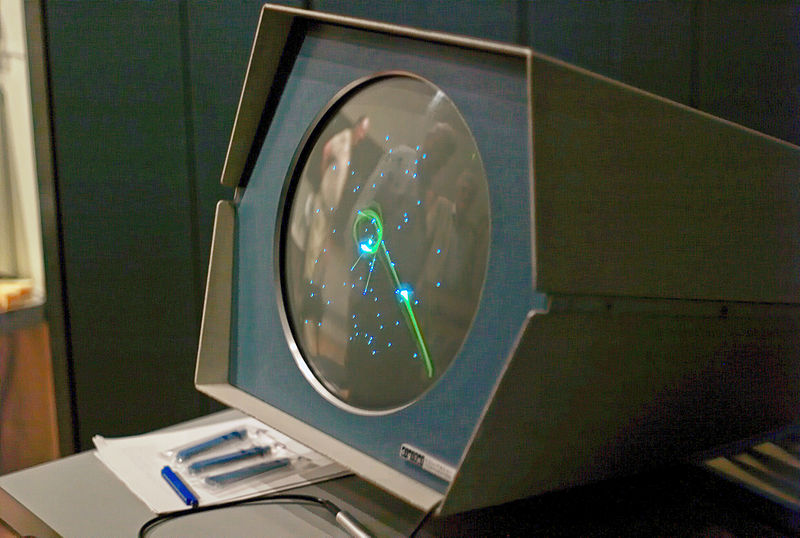
\includegraphics[width=100mm]{Spacewar!.jpg}
\caption{Spacewar! Image from the Wikimedia foundation. http://en.wikipedia.org/wiki/File:Spacewar!-PDP-1-20070512.jpg}
\end{figure}

Hackers are the origin of the concept of a video game. Without the MIT hackers and their Spacewar! game, we might have never seen an industry that quickly eclipsed Hollywood and an art form that is quickly becoming an accepted and powerful medium for a new kind of interactive storytelling.  I strongly recommend that you go see a demo Spacewar! in person at the Museum in Mountain View before you pass any judgement about it's aesthetic value. This photograph doesn't capture the certain glow of those phosphors.

\begin{figure}[ht!]
\center
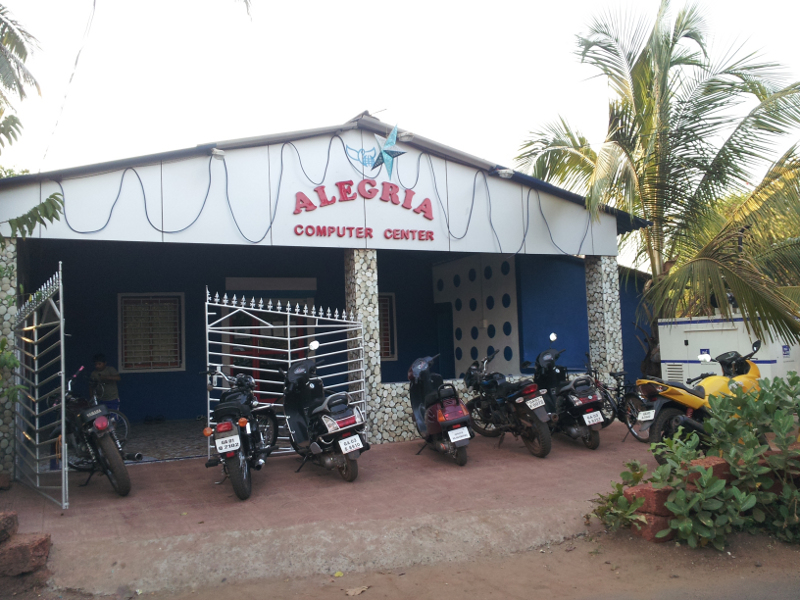
\includegraphics[width=100mm]{alegria_outside.jpg}
\caption{Alegria LAN Center, outside. Vagator, Goa - March 5th, 2013}
\end{figure}

Anyway, the last thing I expected to do during my week in Goa was to play Call of Duty 4 with a bunch of locals (and a few Russians, since North Goa is filled with Russians. There's even Cyrillic writing on some of the signboards and menus). But I guess when I focus so much on a certian aspect of Indian culture, I find what I'm looking for even when I'm not trying to. The place is quite secured from any possible issues, there is a backup generator to keep things running in case of power outage, and a sophisticated, professional power system put in place. Honestly, it's a slick setup. There are about a dozen PC's, ten of which are set up for gaming\footnote{Intel i3 processors, 4GB RAM, 1GB of ram on the video cards, 500GB hard drives. These are not top of the line machines, but they can play the newest games without any trouble. I wouldn't mind putting a machine like one of these together to play the game I'm a little hooked on now.}, and the others for basic web browsing. There's also a side-room that has a couple or three big screen TV's with some game consoles. I didn't check which ones.

\begin{figure}[ht!]
\center
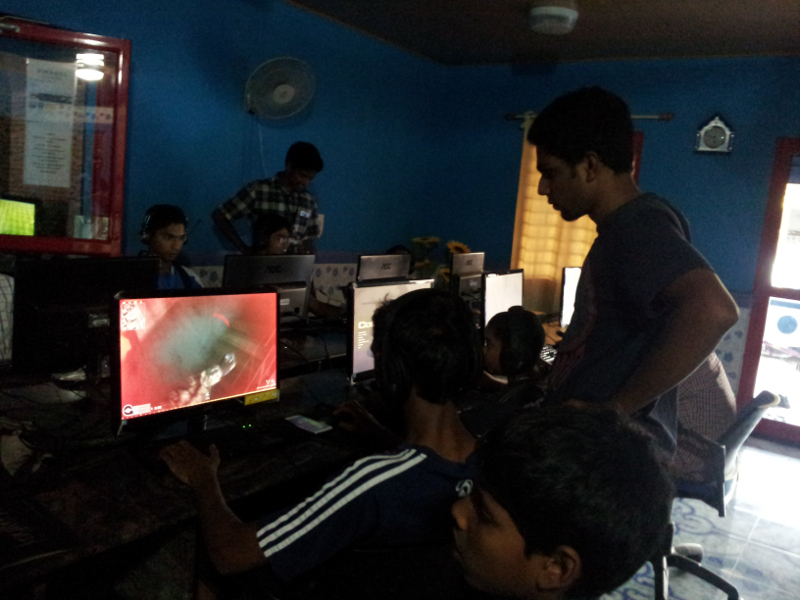
\includegraphics[width=100mm]{alegria_inside.jpg}
\caption{Alegria LAN Center, inside. Vagator, Goa - March 5th 2013}
\end{figure}

The group game of choice happened to be Call of Duty 4, Modern Warfare, played as a deathmatch free for all. The participants were hooting and hollering as they skillfully snuck around the virtual battlefield filling each other's avatars with simulated bullets. I lost, badly, twice, and decided to play something else for a while. The computers are loaded with a cache of recent games, just about every major AAA title that came out in the past few years. I'm currently hooked on a title called Prototype 2, which is a game where you play as soldier who becomes some kind of genetically engineered bioweapon. It's set in a New York City's dystopic future and has a compelling, if formulaic story, but what would you expect from an action title? I'm going to head over there this afternoon and play some more.

\section{Mar 10 - E-mail with Yatin of Moonlighting}

What were your plans when you started the space? Two years ago, correct?

[YT] 2 years back when this place was started, it was an open community space which expected people to come forward, use the common facilities and also ensure the upkeep of the space. However over last 2 years it transformed from being an open community to a semi-private community where people ensure that they are paying up on time to cover all the rentals and expenses of the space and are also able to enjoy the benefits of interacting with other Moonlighting members.

You mentioned that the house was going to go to other use? Keeping this house as a single unit was a driving factor? What was going to happen to this house otherwise?

[YT] Since there was not too much involvement of people coming to the house, this house was being shut down. But this space always had the charm due to its potential to attract diversity. Over the last 2 years that what we developed and also made the place sustainable.

How did you come upon this space?

[YT] The space was designed by my friend Jacob who was in Delhi to setup his business about 2 years back.

Many hackerspaces teach classes on a regular basis or have electronics workshops? Do you have plans to expand with that kind of direction in mind? Would that be possible here or would you have to get another location for that?

[YT] Well we have too many things already going on within the house. Since it is a resident cum coworking space, it becomes difficult to manage too many activities together. We do not want to distract our coworkers or residents too much due to which we do limited events but focus more on our internal gatherings.

What are your plans for the future of Moonlighting?

[YT] We are exploring the opportunity of Franchising Moonlighting for other locations, besides that we are trying to figure out a plan to grow coworking network using our existing technology.

Moonlighting might be the only guesthouse (commune?) that's also a hackerspace, are you connected with other communes in this area of the world as well?

[YT] Yes Moonlighting is the online house cum cowork space in India as of now. Jaaga has some elements of our space but both are very different. It is more of an open space and targets artists, while our focus is more on building entrepreneurs and social enterprise.

\section{Mar 10 - Diwali in Bangalore}

\end{document}